\chapter{Generierung von Zufallszahlen}

Dieses Kapitel behandelt Grundlagen und Methoden zur Generierung von beliebig
verteilten Zufallszahlen durch einen Zufallszahlengenerator mit gleichverteilten
Zufallszahlen.

\section{Zufallsvektoren}

\begin{definition}{Zufallsvektor}{zvektor}
Seien $X_1, ..., X_n$ \link{def:zvar}{Zufallsvariablen}. Die Zusammenfassung
\[\underline{X} = (X_1, ..., X_n)^T\]
zu einem Vektor heißt \defw{Zufallsvektor}. Sind alle Komponenten des Vektors
diskret beziehungsweise stetig, heißt der Zufallsvektor diskret beziehungsweise
stetig.
\end{definition}

Die Werte eines (zweidimensionalen) diskreten Zufallsvektors lassen sich in einer Matrix
zusammenfassen:

\begin{definition}{Gemeinsame Verteilung eines Zufallsvektors}{vert-zvektor}
Sei $\underline{X} = (X, Y)^T$ ein diskreter Zufallsvektor, wobei die
Zufallsvariable $X$ die Werte $x_0, x_1, ..., x_n$ und $Y$ die Werte $y_0, y_1, ...,
y_m$ annimmt. Dann bezeichnet die Matrix
\[(p_{ij})_{i=0,...,n;j=0,...,m} \qquad mit\ p_{ij} = P(X=x_i, Y=y_j)\]
die \defw{gemeinsame Verteilung} von $\underline{X}$.
\end{definition}

Die Summierung von Zeilen bzw. Spalten der Matrix werden als Randverteilung
bezeichnet:
\[p_{i.}:=P(X=x_i) = \sum_j p_{ij}\]
\[p_{.j}:=P(Y=y_j) = \sum_i p_{ij}\]
Für stetige Zufallsvariablen $X$ und $Y$ mit gemeinsamer \link{def:dichte}{Dichte}
$\rho_{(X, Y)}\ge 0$ können folgende \defw{Randdichten} abgeleitet werden:
\[\rho_X(x) = \int\rho_{(X,Y)}(x,y)\mathrm{d} y\quad x\in\R\]
\[\rho_Y(y) = \int\rho_{(X,Y)}(x,y)\mathrm{d} x\quad y\in\R\]

Analog zur \link{def:bedw}{bedingten Wahrscheinlichkeit} von Ereignissen lässt sich
auch für Zufallsvektoren eine bedingte Wahrscheinlichkeit definieren:

\begin{definition}{Bedingte Wahrscheinlichkeit/Bedingte Dichte}{bwahr-zvektor}
Sei $\underline{X} = (X, Y)^T$ ein diskreter Zufallsvektor mit
\link{def:vert-zvektor}{gemeinsamer Verteilung} $(p_{ij})_{i,j=0,1,...}$. Dann ist
mit
\[P(Y=y_j|X=x_i) := \frac{P(X=x_i, Y=y_j)}{P(X=x_i)} = \frac{p_{ij}}{p_{i.}}\]
die \defw{bedingte Wahrscheinlichkeit} von $Y=y_j$ unter Bedingung $X=x_i$ gegeben.

Ist $\underline{X}$ ein stetiger Zufallsvektor mit gemeinsamer Dichte
$\rho_{(X,Y)}$, so bezeichnen die Funktionen
\[\rho_{X|Y=y}(x) = \frac{\rho_{(X,Y)}(x,y)}{\rho_Y(y)}\]
\[\rho_{Y|X=x}(y) = \frac{\rho_{(X,Y)}(x,y)}{\rho_X(x)}\]
die \defw{bedingte Dichte} von $X$ unter $Y=y$ bzw. $Y$ unter $X=x$.
\end{definition}

Ebenso analog zur \link{def:bedw}{bedingten Wahrscheinlichkeit} von Ereignissen kann
der \link{satz:bayes}{Satz von Bayes} für diskrete bzw. stetige Zufallsvektoren
formuliert werden:
\[p_{ij} = P(Y=y_j|X=x_i)\cdot p_{i.}\]
\[\rho_{(X,Y)} = \rho_{Y|X=x}(y)\cdot\rho_X(x)\]

\section{Inversionsmethode}

\begin{theorem}{Transformationssatz}{trafo}
Sei $X$ eine stetige Zufallsvariable mit \link{def:dichte}{Dichte} $\rho_X$ und
Zustandsraum $S$. Sind $a,b\in\R$ und $a \ne 0$, so besitzt die Zufallsvariable
$Y = a\cdot X + b$ die Dichte
\[\rho_Y(z) = \rho_X\Big(\frac{z-b}{a}\Big)\]
Ist die Funktion $g:S\to\R$ streng monoton, so hat die Zufallsvariable $Y=g(X)$
die Dichte
\[\rho_Y(z) = \rho_X\big(g^{-1}(z)\big)\cdot\big|\big(g^{-1}\big)^\prime(z)\big|\]
\end{theorem}

Die Wahrscheinlichkeitsdichte einer verteilte Zufallsvariable $Y$ kann auf die
Wahrscheinlichkeitsdichte einer anderen Zufallsvariable $X$ zurückgeführt
werden. Genau das wenden wir jetzt mit der Inversionsmethode an: Die
Zufallsvariable $Y$ soll eine beliebige Verteilung besitzten, die wir aus
gleichverteilten Zufallszahlen erzeugen. Dafür benötigen wir nur noch eine
geeignete Funktion $g$, sodass $Y=g(X)$ gilt. Das erreichen wir durch das
Inverse der Verteilungsfunktion:

\begin{theorem}{Inversionsmethode}{inversionsm}
Sei $U\sim U(0,1)$ eine gleichverteilte Zufallsvariable und $Y$ eine
beliebige stetige Zufallsvariable mit \link{def:vertf}{Verteilungsfunktion}
$F_Y$. Dann gilt:
\[F_Y^{-1}(U) \sim Y\]
\end{theorem}

\begin{example}{Exponentialverteilung}{exp}
Wir wollen Zufallszahlen $X\sim Exp(\alpha)$ erzeugen. $X$ besitzt die Dichte
\[
\rho(x) = \begin{cases}
\alpha \e^{-\alpha x} & x > 0 \\
0 & \text{sonst}
\end{cases}
\]
mit der Verteilungsfunktion
\[
F_X(z) = \begin{cases}
1- \e^{-\alpha z} & z > 0 \\
0 & \text{sonst}
\end{cases}
\]
Bei Einschränkung der Verteilungsfunktion auf den Zustandsraum $(0, \infty)$ von
$X$ ergibt sich:
\[F_X: (0,\infty)\to(0,1):x\mapsto1-\e^{-\alpha x}\]

Durch Umstellen ergibt sich folgende Vorschrift für die Umkehrfunktion:
\[F_X^{-1}(y) = -\frac{1}{\alpha} \mathrm{ln}(1-y)\]

Damit können wir mit der Inversionsmethode aus einer gleichverteilten
Zufallsvariable $U$ Zufallszahlen erzeugen, die wie $X$ verteilt sind:
\[F_X^{-1}(U) = -\frac{1}{\alpha} \mathrm{ln}(1-U) \sim X\]

\end{example}

Die Inversionsmethode ist ein effizientes Verfahren, um beliebig verteilte
Zufallszahlen zu erzeugen. Problematisch ist jedoch, dass wir die
Verteilungsfunktion invertieren müssen, was nicht immer möglich ist.

\section{Annahme-Verwerfungs-Methode}

\begin{wrapfigure}{r}{0.5\textwidth}
\centering
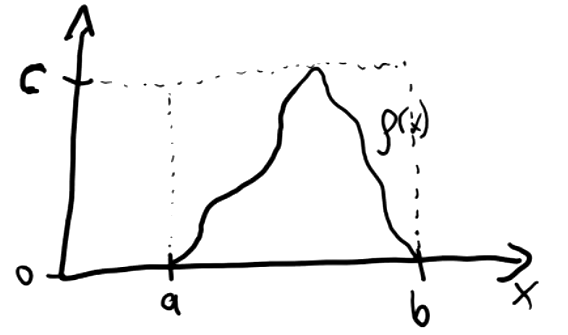
\includegraphics[width=0.4\textwidth]{av-methode}
\end{wrapfigure}
Die Annahme-Verwerfungs-Methode ist ein geometrischer Ansatz, der zufällig
Punkte in einem rechteckigen Bereich generiert, der die
\link{def:dichte}{Dichtefunktion} der gewünschten Verteilung einrahmt.
Notwendige Voraussetzung dafür ist, dass ein endlich großes, die Dichtefunktion
umgebendes Rechteck gefunden werden kann.

Die zufälligen Punkte werden durch skalierte, gleichverteilte Zufallszahlen
bestimmt. Liegt der Punkt unterhalb des Graphs der Dichtefunktion, wird der
X-Wert des Punkts ausgegeben. Damit entspricht die Wahrscheinlichkeit, dass ein
bestimmter Wert als Zufallszahl ausgegeben wird, genau dem Wert der
Wahrscheinlichkeitsdichte an diesem Punkt.

Der folgende Algorithmus gibt eine Folge von Zufallszahlen in der gewünschten
Verteilung aus:

\begin{algorithm}[h!]
\DontPrintSemicolon
\LinesNumbered

\While{1}{
  Erzeuge $x\sim U(a,b)$\;
  Erzeuge $y\sim U(0,1)$\;
  \If{$y\cdot c \le \rho(x)$}{
    gib $x$ aus\;
  }
}


\caption{Annahme-Verwerfungs-Methode}\label{algo:av-methode}
\end{algorithm}

\subsection{Importance-Sampling}

Die Annahme-Verwerfungs-Methode funktioniert dann besonders gut, wenn die Fläche
unter der Dichtefunktion im Vergleich zum einhüllenden Rechteck möglichst gering
ist. In diesem Fall liegen nur wenige Punkte oberhalb der Dichte und müssen
verworfen werden. Ist das einhüllende Rechteck im Vergleich jedoch sehr groß,
beispielsweise weil die Wahrscheinlichkeitsdichte sehr ungleich verteilt ist,
werden viele Punkte verworfen, sodass mehr Zeit für die Erzeugung einer festen
Anzahl an Zufallszahlen erforderlich ist.

Beim Importance-Sampling wird statt eines einhüllenden Rechtecks eine einhüllende
Funktion $h(x)$ verwendet, die weniger Platz als das Rechteck "`verschwendet"'.
Dafür ersetzen wir in Algorithmus \ref{algo:av-methode} die obere Schranke $c$
durch den Wert der Einhüllenden $h(x)$.

Da die Einhüllende $h(x)$ jedoch im Allgmeinen nicht konstant ist, müssen wir
diese Verzerrung korrigieren. Dafür generieren wir die x-Werte der zufälligen
Punkte in der Verteilung der Einhüllenden. Die Einhüllende $h(x)$ besitzt
folgende \link{def:dichte}{Dichte}:
\[H(z) = \frac{1}{\gamma}\cdot\int_a^z h(x) \mathrm{d}x\]
Die Konstante $\gamma = \int_a^b h(x)\mathrm{d}x$ stellt die Normiertheit sicher.

Durch die Inverse $H^{-1}$ der Verteilungsfunktion können mit der
\link{satz:inversionsm}{Inversionsmethode} der Einhüllenden entsprechend
verteilte Zufallszahlen erzeugt werden (da $h(x)$ frei gewählt werden kann, ist
das Invertieren in der Regel kein Problem).

Der entsprechende Algorithmus sieht dann so aus:

\begin{algorithm}[h!]
\DontPrintSemicolon
\LinesNumbered

\While{1}{
  Erzeuge $u\sim U(a,b)$\;
  Setze $x = H^{-1}(u)$\;
  Erzeuge $y\sim U(0,1)$\;
  \If{$y\cdot h(x) \le \rho(x)$}{
    gib $x$ aus\;
  }
}

\caption{Annahme-Verwerfungs-Methode mit Importance Sampling}\label{algo:av-methode-is}
\end{algorithm}

\section{Box-Müller-Polarmethode}

TODO
